\documentclass{ximera}
%% handout
%% nohints
%% space
%% newpage
%% numbers


\prerequisites{none}

\title{1.3 The Derivative at a Point}

\begin{document}
\begin{abstract}
We define the derivative of a function at a point.
\end{abstract}
\maketitle

\section{Overview}

Up next in our discussions is the definition of the foundational idea of nearly all first semester calculus:  the \emph{derivative} of a function at a point.    The derivative is all about change that is happening \emph{instantaneously}, and that instantaneous rate is the limit of corresponding average rates.  In the section, we define the derivative of a function at a point in terms of average rates of change and limits, introduce the ``prime'' notation for the derivative, discuss the units of measurement for the derivative, and connect the derivative to the geometric concept of a tangent line and especially its slope. 


\section{Basic learning objectives}

These are the tasks you should be able to perform with reasonable fluency \textbf{when you arrive at our next class meeting}. Important new vocabulary words are indicated \emph{in italics}. 

\begin{itemize}
	\item Calculate the average rate of change in a function on an interval. 
	\item State the definition of the derivative of a function at a point. 
	\item Use correct notation to indicate the derivative of a function at a point and explain the difference between the quantities $f(a)$ and $f'(a)$. 
	\item Given the units of a function $f$ and the units of an input $a$, state the units of the derivative $f'(a)$.
	\item Describe the derivative in terms of the slope of a tangent line. 
\end{itemize}

\section{Advanced learning objectives}

In addition to mastering the basic objectives, here are the tasks you should be able to perform \textbf{after class, with practice}: 

\begin{itemize}
	\item Give several different interpretations of the meaning of the value $f'(a)$, for a given function $f$ and value $a$.
	\item Use the limit definition of the derivative to compute $f'(a)$ for a variety of different functions $f$ and for any value of $a$.
	\item Be able to explain how the tangent line at a point on a  smooth curve results from taking the limit of appropriate secant lines.
\end{itemize}

\section{Resources}

\noindent
\emph{Reading}: Read Section 1.3, pages 20--28 in Active Calculus.

\noindent
\emph{Watching}: Here are some additional resources that have been developed to support your learning: 

\begin{itemize}
	\item Screencast 1.3.1: \youtube{http://gvsu.edu/s/qJ} 
	\item Screencast 1.3.2: \youtube{http://gvsu.edu/s/qK} 
	\item Screencast 1.3.3: \youtube{http://gvsu.edu/s/qL}
\end{itemize}

\subsection*{Questions}

\noindent Complete each question below.  

\begin{question}
Suppose that $f$ is the function given by the graph below and that $a$ and $a+h$ are the input values as labeled on the $x$-axis.  Use the graph in Figure~\ref{F:1.3.PA1} to answer the following questions.

\begin{figure}[h]
\begin{center}
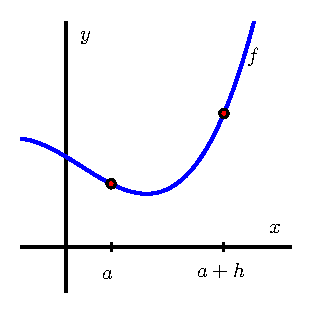
\includegraphics{figures/1_3_PA1.pdf}
\caption{Plot of $y = f(x)$ for Preview Activity~\ref{PA:1.3}.} \label{F:1.3.PA1}
\end{center}
\end{figure}
Copy the graph. Locate and label the points $(a,f(a))$ and $(a+h, f(a+h))$ on the graph.

Construct a right triangle whose hypotenuse is the line segment from $(a,f(a))$ to \\ $(a+h,f(a+h))$. The length of the horizontal leg is \answer{h}.
The length of the vertical leg is 
\begin{multipleChoice}
\choice{$a$}
\choice{$h$}
\choice[correct]{$f(a+h)-f(a)$}
\choice{$f(h)$}
\end{multipleChoice}

What is the slope of the line that connects the points $(a,f(a))$ and $(a+h, f(a+h))$?
\begin{multipleChoice}
\choice{$\frac{a}{h}$}
\choice{$\frac{f(h)}{h}$}
\choice[correct]{$\frac{f(a+h)-f(a)}{h}$}
\choice{$\frac{f(a)}{h}$}
\end{multipleChoice}

Write a meaningful sentence that explains how the average rate of change of the function on a given interval and the slope of a related line are connected.
\begin{freeResponse}
The average rate of change ...
\end{freeResponse}

\end{question}




\end{document}